\begin{enumerate}[label=\thechapter.\arabic*,ref=\thechapter.\theenumi]
\item The network shown below has a resonant frequency of 150 kHz and bandwidth of 600
Hz. The Q-factor of the network is \rule{1cm}{0.15mm}\\
(rounded off to one decimal place).\\
\hfill(GATE 2022 EC)\\
\begin{figure}[ht]
  \centering
  
      \input{2022/EE/28/figs/ckt1}
  
  \caption{Circuit 1}
\end{figure}\\
\solution\\
\iffalse
\let\negmedspace\undefined
\let\negthickspace\undefined
\documentclass[journal,12pt,twocolumn]{IEEEtran}
\usepackage{cite}
\usepackage{amsmath,amssymb,amsfonts,amsthm}
\usepackage{algorithmic}
\usepackage{graphicx}
\usepackage{textcomp}
\usepackage{xcolor}
\usepackage{txfonts}
\usepackage{listings}
\usepackage{enumitem}
\usepackage{mathtools}
\usepackage{gensymb}
\usepackage{comment}
\usepackage[breaklinks=true]{hyperref}
\usepackage{tkz-euclide} 
\usepackage{listings}
\usepackage{gvv}                                        
\def\inputGnumericTable{}                                 
\usepackage[latin1]{inputenc}                                
\usepackage{color}                                            
\usepackage{array}                                            
\usepackage{longtable}                                       
\usepackage{calc}                                             
\usepackage{multirow}                                         
\usepackage{hhline}                                           
\usepackage{ifthen}                                           
\usepackage{lscape}
\usepackage[center]{caption} % center the captions to figure

\newtheorem{theorem}{Theorem}[section]
\newtheorem{problem}{Problem}
\newtheorem{proposition}{Proposition}[section]
\newtheorem{lemma}{Lemma}[section]
\newtheorem{corollary}[theorem]{Corollary}
\newtheorem{example}{Example}[section]
\newtheorem{definition}[problem]{Definition}
\newcommand{\BEQA}{\begin{eqnarray}}
\newcommand{\EEQA}{\end{eqnarray}}
\newcommand{\define}{\stackrel{\triangle}{=}}
\theoremstyle{remark}
\newtheorem{rem}{Remark}
\begin{document}

\newcolumntype{M}[1]{>{\centering\arraybackslash}m{#1}}
\newcolumntype{N}{@{}m{0pt}@{}}

\bibliographystyle{IEEEtran}
\vspace{3cm}

\title{GATE 2021 ME 3Q} 
\author{ee23btech11223 - Soham Prabhakar More% <-this % stops a space
}
\maketitle
\newpage
\bigskip

\renewcommand{\thefigure}{\theenumi}
\renewcommand{\thetable}{\theenumi}

\bibliographystyle{IEEEtran}

\textbf{Question:} The Dirac-delta function $\brak{\delta\brak{t - t_0}}$ for $t, t_0 \in \Re$, has the following property
\begin{align}
    \int_{a}^{b}\phi\brak{t}\delta\brak{t - t_0}dt = 
    \begin{cases}
        \phi\brak{t_0}\quad a < t_0 < b\\
        0 \quad\quad otherwise
    \end{cases} \label{eq:2022.ME.3.1}
\end{align}

The Laplace Transform of the Dirac-delta function $\delta\brak{t - a}$ for $a > 0; \mathcal{L}\brak{\delta\brak{t - a}} = F\brak{s}$ is

\hfill{(GATE 2021 ME 3Q)}

\solution
\fi
\begin{table}[ht]
    \renewcommand\thetable{1}
\begin{tabular}{|c|c|}
    \hline 
    \textbf{Parameter}&\textbf{Description} \\
    \hline
    $F\brak{s}$ & Laplace transform of $\delta\brak{t - a}$ \\
    \hline
    $G\brak{f}$ & Fourier transform of $\delta\brak{t - a}$ \\
    \hline
    $H\brak{t}$ & Fourier transform of a function with period $T$ \\
    \hline
    $w_T\brak{t}$ & Delta Comb, $\sum_{k = -\infty}^{\infty}\delta\brak{t - kT}$ \\
    \hline
    $W_T\brak{t}$ & Fourier transform of $w_T\brak{t}$ \\
    \hline
\end{tabular}

\caption{Table of parameters}
\label{Table:2022.ME.3.1}


\end{table} \\

By \eqref{eq:2022.ME.3.1} and $a > 0$,
\begin{align}
    F\brak{s} &= \int_{0}^{\infty}\delta\brak{t - a}e^{-st}dt \\
    \therefore F\brak{s} &= e^{-as}
\end{align}

The fourier transform,
\begin{align}
    G\brak{f} &= \int_{-\infty}^{\infty}\delta\brak{t - a}e^{-2\pi jft}dt \\
    \therefore G\brak{f} &= e^{-j2\pi fa}
\end{align}
For a periodic signal the fourier transform is defined as:
\begin{align}
    H\brak{f} &= \sum_{k = -\infty}^{\infty}c_k\delta\brak{f - \frac{k}{T}}
\end{align}
where $c_k$ are the fourier series coefficients and $T$ is the period. Thus,
\begin{align}
    W_T\brak{f} &= \sum_{k = -\infty}^{\infty}c_k\delta\brak{f - \frac{k}{T}} \\
    c_k &= \frac{1}{T}\int_{-\frac{T}{2}}^{\frac{T}{2}}w_T\brak{t}e^{-j2\pi \frac{k}{T}f}dt \\
    c_k &= \frac{1}{T}\int_{-\frac{T}{2}}^{\frac{T}{2}}\brak{\sum_{k = -\infty}^{\infty}\delta\brak{t - kT}}e^{-j2\pi \frac{k}{T}f}dt \\
\end{align}
\begin{align}
    c_k &= \frac{1}{T}\sum_{k = -\infty}^{\infty}\int_{-\frac{T}{2}}^{\frac{T}{2}}\delta\brak{t - kT}e^{-j2\pi \frac{k}{T}f}dt \\
    c_k &= \frac{1}{T} \\
    W_T\brak{f} &= \frac{1}{T}\sum_{k = -\infty}^{\infty}\delta\brak{f - \frac{k}{T}} \\
    \therefore W_T\brak{f} &= \frac{1}{T}w_{\frac{1}{T}}\brak{f}
\end{align}
Thus, the fourier transform of impulse train is another impulse train.
%\begin{align}
%    f\brak{t} &\system{F} H\brak{f} \\
%    f\brak{t + T} &\system{F} e^{j2\pi fT}H\brak{f} \\
%    \because e^{j2\pi fT}H\brak{f} &= H\brak{f} \\
%    H\brak{f}\brak{1 - e^{j2\pi fT}} &= 0
%\end{align}
%Thus, $H\brak{f}$ is zero everywhere except at $f = \frac{n}{T}, n \in Z$
%\begin{align}
%    \therefore H\brak{f} &= \sum_{k = -\infty}^{\infty}c_k\delta\brak{f - \frac{k}{T}} \\
%    \because \sum_{k = -\infty}^{\infty}c_ke^{-j2\pi f\frac{k}{T}} &\system{F} H\brak{f}
%\end{align}
%$c_k$ are the fourier series coefficents of $h\brak{t}$,
%\begin{align}
%    c_k = \int_{-\frac{T}{2}}^{\frac{T}{2}}
%\end{align}
%\end{document}

\pagebreak
\item A circuit with an ideal OPAMP is shown. The Bode plot for the magnitude (in dB)
 of the gain transfer function $ \brak{A \brak{j \omega}} = \dfrac{ V_{out}\brak{j \omega}}{V_{in}\brak{j \omega}}$ of the circuit is also
provided (here, $\omega$ is the angular frequency in $ rad/s $). The values of $R$ and $C$ are 
\begin{figure}[ht]
	\centering
    \includegraphics[width=\columnwidth]{2022/EC/42/figs/fig1.png}
    \label{fig:2022.42.39}
\end{figure} 
\begin{enumerate}[label = (\Alph*)]
     \item $R$ = $3k\ohm$,  $C$ = $1\mu F$\\
     \item $R$ = $1k\ohm$,  $C$ = $3\mu F$\\
     \item $R$ = $4k\ohm$,  $C$ = $1\mu F$\\
     \item $R$ = $3k\ohm$,  $C$ = $2\mu F$\\
\end{enumerate}
\hfill(GATE 2022 EC)\\
\solution\\
\input{2022/EC/42/ec.tex}
\pagebreak

\item  In the circuit shown, the load is driven by a sinusoidal A.C. voltage source $V_1 = 100\angle0\degree V$ at $50Hz$. Given $R_1 = 20\Omega$, $C_1 = \brak{\frac{1000}{\pi}}\mu F$, $L_1 = \brak{\frac{20}{\pi}}mH$ and $R_2 = 4\Omega$, the power factor is \_\_\_\_\_ (round off to one decimal place)\\
\hfill(GATE 2022 IN Q52)
\input{2022/IN/52/figs/question}
\solution
\input{2022/IN/52/GATE_22_IN_52.tex}
\pagebreak

\item For the circuit shown, the locus of the impedance $ Z\brak{j\omega}$ is plotted as $ \omega$ increases from zero to infinity. The values of $ R_1$ and $ R_2$ are:
\begin{enumerate}
    \item[(A)] $ R_1 = 2\text{ k\ohm}, R_2 = 3\text{ k\ohm}$
    \item[(B)]$ R_1 = 5\text{ k\ohm}, R_2 = 2\text{ k\ohm}$
    \item[(C)] $ R_1 = 5\text{ k\ohm}, R_2 = 2.5\text{ k\ohm}$
    \item[(D)] $ R_1 = 2\text{ k\ohm}, R_2 = 5\text{ k\ohm}$
\end{enumerate}

\begin{figure}[h!]
    \includegraphics[width = 0.6\columnwidth]{2022/EC/38/figs/qn_fig.pdf}
    \caption{Figure of circuit}
    \centering
    \label{fig: ece38_qn_fig}
\end{figure}

\begin{figure}[h!]
    \includegraphics[width = 0.6\columnwidth]{2022/EC/38/figs/fig_2.png}
    \caption{}
    \centering
    \label{fig: ece38qn_2_fig}
\end{figure}
\hfill(GATE ECE 2022 QUESTION 38)\\
\solution
\input{2022/EC/38/asnmt8.tex}
\pagebreak

\item In the bandpass filter circuit shown, $R_0 = 50\Omega$, $L_0 = 1 mH$, $C_0 = 10nF$. The q factor of the filter is 
\input{2022/IN/33/figs/fig_1}
\hfill(GATE 2022 IN Q33)\\
\solution
\iffalse
\let\negmedspace\undefined
\let\negthickspace\undefined
\documentclass[journal,12pt,twocolumn]{IEEEtran}
\usepackage{cite}
\usepackage{amsmath,amssymb,amsfonts,amsthm}
\usepackage{algorithmic}
\usepackage{graphicx}
\usepackage{textcomp}
\usepackage{xcolor}
\usepackage{txfonts}
\usepackage{listings}
\usepackage{enumitem}
\usepackage{mathtools}
\usepackage{gensymb}
\usepackage{comment}
\usepackage[breaklinks=true]{hyperref}
\usepackage{tkz-euclide} 
\usepackage{listings}
\usepackage{gvv}                                        
\def\inputGnumericTable{}                                 
\usepackage[latin1]{inputenc}                                
\usepackage{color}                                            
\usepackage{array}                                            
\usepackage{longtable}                                       
\usepackage{calc}                                             
\usepackage{multirow}                                         
\usepackage{hhline}                                           
\usepackage{ifthen}                                           
\usepackage{lscape}
\usepackage[center]{caption} % center the captions to figure

\newtheorem{theorem}{Theorem}[section]
\newtheorem{problem}{Problem}
\newtheorem{proposition}{Proposition}[section]
\newtheorem{lemma}{Lemma}[section]
\newtheorem{corollary}[theorem]{Corollary}
\newtheorem{example}{Example}[section]
\newtheorem{definition}[problem]{Definition}
\newcommand{\BEQA}{\begin{eqnarray}}
\newcommand{\EEQA}{\end{eqnarray}}
\newcommand{\define}{\stackrel{\triangle}{=}}
\theoremstyle{remark}
\newtheorem{rem}{Remark}
\begin{document}

\newcolumntype{M}[1]{>{\centering\arraybackslash}m{#1}}
\newcolumntype{N}{@{}m{0pt}@{}}

\bibliographystyle{IEEEtran}
\vspace{3cm}

\title{GATE 2021 ME 3Q} 
\author{ee23btech11223 - Soham Prabhakar More% <-this % stops a space
}
\maketitle
\newpage
\bigskip

\renewcommand{\thefigure}{\theenumi}
\renewcommand{\thetable}{\theenumi}

\bibliographystyle{IEEEtran}

\textbf{Question:} The Dirac-delta function $\brak{\delta\brak{t - t_0}}$ for $t, t_0 \in \Re$, has the following property
\begin{align}
    \int_{a}^{b}\phi\brak{t}\delta\brak{t - t_0}dt = 
    \begin{cases}
        \phi\brak{t_0}\quad a < t_0 < b\\
        0 \quad\quad otherwise
    \end{cases} \label{eq:2022.ME.3.1}
\end{align}

The Laplace Transform of the Dirac-delta function $\delta\brak{t - a}$ for $a > 0; \mathcal{L}\brak{\delta\brak{t - a}} = F\brak{s}$ is

\hfill{(GATE 2021 ME 3Q)}

\solution
\fi
\begin{table}[ht]
    \renewcommand\thetable{1}
\begin{tabular}{|c|c|}
    \hline 
    \textbf{Parameter}&\textbf{Description} \\
    \hline
    $F\brak{s}$ & Laplace transform of $\delta\brak{t - a}$ \\
    \hline
    $G\brak{f}$ & Fourier transform of $\delta\brak{t - a}$ \\
    \hline
    $H\brak{t}$ & Fourier transform of a function with period $T$ \\
    \hline
    $w_T\brak{t}$ & Delta Comb, $\sum_{k = -\infty}^{\infty}\delta\brak{t - kT}$ \\
    \hline
    $W_T\brak{t}$ & Fourier transform of $w_T\brak{t}$ \\
    \hline
\end{tabular}

\caption{Table of parameters}
\label{Table:2022.ME.3.1}


\end{table} \\

By \eqref{eq:2022.ME.3.1} and $a > 0$,
\begin{align}
    F\brak{s} &= \int_{0}^{\infty}\delta\brak{t - a}e^{-st}dt \\
    \therefore F\brak{s} &= e^{-as}
\end{align}

The fourier transform,
\begin{align}
    G\brak{f} &= \int_{-\infty}^{\infty}\delta\brak{t - a}e^{-2\pi jft}dt \\
    \therefore G\brak{f} &= e^{-j2\pi fa}
\end{align}
For a periodic signal the fourier transform is defined as:
\begin{align}
    H\brak{f} &= \sum_{k = -\infty}^{\infty}c_k\delta\brak{f - \frac{k}{T}}
\end{align}
where $c_k$ are the fourier series coefficients and $T$ is the period. Thus,
\begin{align}
    W_T\brak{f} &= \sum_{k = -\infty}^{\infty}c_k\delta\brak{f - \frac{k}{T}} \\
    c_k &= \frac{1}{T}\int_{-\frac{T}{2}}^{\frac{T}{2}}w_T\brak{t}e^{-j2\pi \frac{k}{T}f}dt \\
    c_k &= \frac{1}{T}\int_{-\frac{T}{2}}^{\frac{T}{2}}\brak{\sum_{k = -\infty}^{\infty}\delta\brak{t - kT}}e^{-j2\pi \frac{k}{T}f}dt \\
\end{align}
\begin{align}
    c_k &= \frac{1}{T}\sum_{k = -\infty}^{\infty}\int_{-\frac{T}{2}}^{\frac{T}{2}}\delta\brak{t - kT}e^{-j2\pi \frac{k}{T}f}dt \\
    c_k &= \frac{1}{T} \\
    W_T\brak{f} &= \frac{1}{T}\sum_{k = -\infty}^{\infty}\delta\brak{f - \frac{k}{T}} \\
    \therefore W_T\brak{f} &= \frac{1}{T}w_{\frac{1}{T}}\brak{f}
\end{align}
Thus, the fourier transform of impulse train is another impulse train.
%\begin{align}
%    f\brak{t} &\system{F} H\brak{f} \\
%    f\brak{t + T} &\system{F} e^{j2\pi fT}H\brak{f} \\
%    \because e^{j2\pi fT}H\brak{f} &= H\brak{f} \\
%    H\brak{f}\brak{1 - e^{j2\pi fT}} &= 0
%\end{align}
%Thus, $H\brak{f}$ is zero everywhere except at $f = \frac{n}{T}, n \in Z$
%\begin{align}
%    \therefore H\brak{f} &= \sum_{k = -\infty}^{\infty}c_k\delta\brak{f - \frac{k}{T}} \\
%    \because \sum_{k = -\infty}^{\infty}c_ke^{-j2\pi f\frac{k}{T}} &\system{F} H\brak{f}
%\end{align}
%$c_k$ are the fourier series coefficents of $h\brak{t}$,
%\begin{align}
%    c_k = \int_{-\frac{T}{2}}^{\frac{T}{2}}
%\end{align}
%\end{document}

\pagebreak

\item In the circuit shown below, the switch S is closed at $t=0$. The magnitude of the steady state voltage, in volts, across the $6\Omega$ resistor is \_\_\_\_\_.(\textit{round off to two decimal places})\\ \hfill(GATE 2022 EE Q31)
\input{2022/EE/31/figs/question}\\
\solution
\input{2022/EE/31/GATE_2022_EE_31.tex}
\pagebreak

\item An ideal OPAMP circuit with a sinusoidal input is shown in the figure. The 3dB frequency is the frequency at which the magnitude of the voltage gain decreases by 3 dB from the maximum value. Which of the options is/are correct?

\begin{figure}[H]
  \centering
  \input{2022/EC/26/codes/circuit1.tex}
  \label{fig:26fig1}
\end{figure}

\begin{enumerate}[label=(\Alph*)]
\item The circuit is a low pass filter.\\
\item The circuit is a high pass filter.\\
\item The 3 dB frequency is 1000rad/s.\\
\item The 3 dB frequency is $\frac{1000}{3}$rad/s.\\
\end{enumerate}
\hfill(GATE EC 2022)\\
\solution
\input{2022/EC/26/gate22.tex}
\pagebreak

\item A series $RLC$ circuit with $R = 10 \Omega$, $L = 50 mH$ and $C = 100 \micro F$ connected to
$200$ $V$, $50$ Hz supply consumes power $P$. The value of $L$ is changed such that this
circuit consumes same power $P$ but operates with lagging power factor. The new
value of L is $\hrulefill$ $mH$ (rounded off to two decimal places).
\hfill(GATE 33 BM 2022)

\solution
\iffalse
\let\negmedspace\undefined
\let\negthickspace\undefined
\documentclass[journal,12pt,twocolumn]{IEEEtran}
\usepackage{cite}
\usepackage{amsmath,amssymb,amsfonts,amsthm}
\usepackage{algorithmic}
\usepackage{graphicx}
\usepackage{textcomp}
\usepackage{xcolor}
\usepackage{txfonts}
\usepackage{listings}
\usepackage{enumitem}
\usepackage{mathtools}
\usepackage{gensymb}
\usepackage{comment}
\usepackage[breaklinks=true]{hyperref}
\usepackage{tkz-euclide} 
\usepackage{listings}
\usepackage{gvv}                                        
\def\inputGnumericTable{}                                 
\usepackage[latin1]{inputenc}                                
\usepackage{color}                                            
\usepackage{array}                                            
\usepackage{longtable}                                       
\usepackage{calc}                                             
\usepackage{multirow}                                         
\usepackage{hhline}                                           
\usepackage{ifthen}                                           
\usepackage{lscape}
\usepackage[center]{caption} % center the captions to figure

\newtheorem{theorem}{Theorem}[section]
\newtheorem{problem}{Problem}
\newtheorem{proposition}{Proposition}[section]
\newtheorem{lemma}{Lemma}[section]
\newtheorem{corollary}[theorem]{Corollary}
\newtheorem{example}{Example}[section]
\newtheorem{definition}[problem]{Definition}
\newcommand{\BEQA}{\begin{eqnarray}}
\newcommand{\EEQA}{\end{eqnarray}}
\newcommand{\define}{\stackrel{\triangle}{=}}
\theoremstyle{remark}
\newtheorem{rem}{Remark}
\begin{document}

\newcolumntype{M}[1]{>{\centering\arraybackslash}m{#1}}
\newcolumntype{N}{@{}m{0pt}@{}}

\bibliographystyle{IEEEtran}
\vspace{3cm}

\title{GATE 2021 ME 3Q} 
\author{ee23btech11223 - Soham Prabhakar More% <-this % stops a space
}
\maketitle
\newpage
\bigskip

\renewcommand{\thefigure}{\theenumi}
\renewcommand{\thetable}{\theenumi}

\bibliographystyle{IEEEtran}

\textbf{Question:} The Dirac-delta function $\brak{\delta\brak{t - t_0}}$ for $t, t_0 \in \Re$, has the following property
\begin{align}
    \int_{a}^{b}\phi\brak{t}\delta\brak{t - t_0}dt = 
    \begin{cases}
        \phi\brak{t_0}\quad a < t_0 < b\\
        0 \quad\quad otherwise
    \end{cases} \label{eq:2022.ME.3.1}
\end{align}

The Laplace Transform of the Dirac-delta function $\delta\brak{t - a}$ for $a > 0; \mathcal{L}\brak{\delta\brak{t - a}} = F\brak{s}$ is

\hfill{(GATE 2021 ME 3Q)}

\solution
\fi
\begin{table}[ht]
    \renewcommand\thetable{1}
\begin{tabular}{|c|c|}
    \hline 
    \textbf{Parameter}&\textbf{Description} \\
    \hline
    $F\brak{s}$ & Laplace transform of $\delta\brak{t - a}$ \\
    \hline
    $G\brak{f}$ & Fourier transform of $\delta\brak{t - a}$ \\
    \hline
    $H\brak{t}$ & Fourier transform of a function with period $T$ \\
    \hline
    $w_T\brak{t}$ & Delta Comb, $\sum_{k = -\infty}^{\infty}\delta\brak{t - kT}$ \\
    \hline
    $W_T\brak{t}$ & Fourier transform of $w_T\brak{t}$ \\
    \hline
\end{tabular}

\caption{Table of parameters}
\label{Table:2022.ME.3.1}


\end{table} \\

By \eqref{eq:2022.ME.3.1} and $a > 0$,
\begin{align}
    F\brak{s} &= \int_{0}^{\infty}\delta\brak{t - a}e^{-st}dt \\
    \therefore F\brak{s} &= e^{-as}
\end{align}

The fourier transform,
\begin{align}
    G\brak{f} &= \int_{-\infty}^{\infty}\delta\brak{t - a}e^{-2\pi jft}dt \\
    \therefore G\brak{f} &= e^{-j2\pi fa}
\end{align}
For a periodic signal the fourier transform is defined as:
\begin{align}
    H\brak{f} &= \sum_{k = -\infty}^{\infty}c_k\delta\brak{f - \frac{k}{T}}
\end{align}
where $c_k$ are the fourier series coefficients and $T$ is the period. Thus,
\begin{align}
    W_T\brak{f} &= \sum_{k = -\infty}^{\infty}c_k\delta\brak{f - \frac{k}{T}} \\
    c_k &= \frac{1}{T}\int_{-\frac{T}{2}}^{\frac{T}{2}}w_T\brak{t}e^{-j2\pi \frac{k}{T}f}dt \\
    c_k &= \frac{1}{T}\int_{-\frac{T}{2}}^{\frac{T}{2}}\brak{\sum_{k = -\infty}^{\infty}\delta\brak{t - kT}}e^{-j2\pi \frac{k}{T}f}dt \\
\end{align}
\begin{align}
    c_k &= \frac{1}{T}\sum_{k = -\infty}^{\infty}\int_{-\frac{T}{2}}^{\frac{T}{2}}\delta\brak{t - kT}e^{-j2\pi \frac{k}{T}f}dt \\
    c_k &= \frac{1}{T} \\
    W_T\brak{f} &= \frac{1}{T}\sum_{k = -\infty}^{\infty}\delta\brak{f - \frac{k}{T}} \\
    \therefore W_T\brak{f} &= \frac{1}{T}w_{\frac{1}{T}}\brak{f}
\end{align}
Thus, the fourier transform of impulse train is another impulse train.
%\begin{align}
%    f\brak{t} &\system{F} H\brak{f} \\
%    f\brak{t + T} &\system{F} e^{j2\pi fT}H\brak{f} \\
%    \because e^{j2\pi fT}H\brak{f} &= H\brak{f} \\
%    H\brak{f}\brak{1 - e^{j2\pi fT}} &= 0
%\end{align}
%Thus, $H\brak{f}$ is zero everywhere except at $f = \frac{n}{T}, n \in Z$
%\begin{align}
%    \therefore H\brak{f} &= \sum_{k = -\infty}^{\infty}c_k\delta\brak{f - \frac{k}{T}} \\
%    \because \sum_{k = -\infty}^{\infty}c_ke^{-j2\pi f\frac{k}{T}} &\system{F} H\brak{f}
%\end{align}
%$c_k$ are the fourier series coefficents of $h\brak{t}$,
%\begin{align}
%    c_k = \int_{-\frac{T}{2}}^{\frac{T}{2}}
%\end{align}
%\end{document}

\pagebreak

\item A single-phase full-bridge diode rectifier feeds a resistive load of $50 \Omega$ from a 200 V,
50 Hz single phase AC supply. If the diodes are ideal, then the active power, in watts,
drawn by the load is \rule{1cm}{0.5mm} (round off to nearest integer).  \\
\hfill (GATE EE 32)\\
\solution
\input{2022/EE/32/gate2.tex}
\pagebreak

\item The circuit shown is driven by a sinusoidal input voltage, $V_{\text{in}}$, resulting in the output voltage $V_{\text{out}}$. The frequency (in kilohertz) at which the voltage gain is 0 dB is (rounded off to two decimal places).
\begin{figure}[htb]
  \centering
  \input{2022/IN/56/figs/fig1.tex}
\end{figure}
\hfill(GATE IN 2022)\\
\solution
\input{2022/IN/56/gate.tex}
\pagebreak

\item An inductor having a $Q$-factor of 60 is connected in series with a capacitor having a $Q$-factor of 240. The overall $Q$-factor of the circuit is \_\_\_\_\_\_\_\_\_\_. (Round off to the nearest integer) \\
\hfill Gate 2022 EE Question 27\\
\solution
\input{2022/EE/27/gate2022.tex}
\pagebreak

\item In the circuit shown, the switch is initially closed. It is opened at t= 0 s and
remains open thereafter. The time (in milliseconds) at which the output voltage
$V_{out}$ becomes LOW is  (round off to three decimal places)\hfill(GATE IN 2022)\\
\input{2022/IN/64/figs/tikzque}
\solution\\
\input{2022/IN/64/gate3.tex}
\pagebreak

\item The steady state output $v_{out}$ of the circuit shown below, will
\begin{figure}[h]
    \centering
    \input{2022/EE/16/figs/ques}
    \caption{Circuit}
    \label{fig: 217.EE.16.1}
\end{figure}

\begin{enumerate}
    \item saturate to $+V_{DD}$
    \item saturate to $-V_{EE}$
    \item become equal to $0.1V$
    \item become equal to $-0.1V$
\end{enumerate}
\solution
\iffalse
\let\negmedspace\undefined
\let\negthickspace\undefined
\documentclass[journal,12pt,twocolumn]{IEEEtran}
\usepackage{cite}
\usepackage{amsmath,amssymb,amsfonts,amsthm}
\usepackage{algorithmic}
\usepackage{graphicx}
\usepackage{textcomp}
\usepackage{xcolor}
\usepackage{txfonts}
\usepackage{listings}
\usepackage{enumitem}
\usepackage{mathtools}
\usepackage{gensymb}
\usepackage{comment}
\usepackage[breaklinks=true]{hyperref}
\usepackage{tkz-euclide} 
\usepackage{listings}
\usepackage{gvv}                                        
\def\inputGnumericTable{}                                 
\usepackage[latin1]{inputenc}                                
\usepackage{color}                                            
\usepackage{array}                                            
\usepackage{longtable}                                       
\usepackage{calc}                                             
\usepackage{multirow}                                         
\usepackage{hhline}                                           
\usepackage{ifthen}                                           
\usepackage{lscape}
\usepackage[center]{caption} % center the captions to figure

\newtheorem{theorem}{Theorem}[section]
\newtheorem{problem}{Problem}
\newtheorem{proposition}{Proposition}[section]
\newtheorem{lemma}{Lemma}[section]
\newtheorem{corollary}[theorem]{Corollary}
\newtheorem{example}{Example}[section]
\newtheorem{definition}[problem]{Definition}
\newcommand{\BEQA}{\begin{eqnarray}}
\newcommand{\EEQA}{\end{eqnarray}}
\newcommand{\define}{\stackrel{\triangle}{=}}
\theoremstyle{remark}
\newtheorem{rem}{Remark}
\begin{document}

\newcolumntype{M}[1]{>{\centering\arraybackslash}m{#1}}
\newcolumntype{N}{@{}m{0pt}@{}}

\bibliographystyle{IEEEtran}
\vspace{3cm}

\title{GATE 2021 ME 3Q} 
\author{ee23btech11223 - Soham Prabhakar More% <-this % stops a space
}
\maketitle
\newpage
\bigskip

\renewcommand{\thefigure}{\theenumi}
\renewcommand{\thetable}{\theenumi}

\bibliographystyle{IEEEtran}

\textbf{Question:} The Dirac-delta function $\brak{\delta\brak{t - t_0}}$ for $t, t_0 \in \Re$, has the following property
\begin{align}
    \int_{a}^{b}\phi\brak{t}\delta\brak{t - t_0}dt = 
    \begin{cases}
        \phi\brak{t_0}\quad a < t_0 < b\\
        0 \quad\quad otherwise
    \end{cases} \label{eq:2022.ME.3.1}
\end{align}

The Laplace Transform of the Dirac-delta function $\delta\brak{t - a}$ for $a > 0; \mathcal{L}\brak{\delta\brak{t - a}} = F\brak{s}$ is

\hfill{(GATE 2021 ME 3Q)}

\solution
\fi
\begin{table}[ht]
    \renewcommand\thetable{1}
\begin{tabular}{|c|c|}
    \hline 
    \textbf{Parameter}&\textbf{Description} \\
    \hline
    $F\brak{s}$ & Laplace transform of $\delta\brak{t - a}$ \\
    \hline
    $G\brak{f}$ & Fourier transform of $\delta\brak{t - a}$ \\
    \hline
    $H\brak{t}$ & Fourier transform of a function with period $T$ \\
    \hline
    $w_T\brak{t}$ & Delta Comb, $\sum_{k = -\infty}^{\infty}\delta\brak{t - kT}$ \\
    \hline
    $W_T\brak{t}$ & Fourier transform of $w_T\brak{t}$ \\
    \hline
\end{tabular}

\caption{Table of parameters}
\label{Table:2022.ME.3.1}


\end{table} \\

By \eqref{eq:2022.ME.3.1} and $a > 0$,
\begin{align}
    F\brak{s} &= \int_{0}^{\infty}\delta\brak{t - a}e^{-st}dt \\
    \therefore F\brak{s} &= e^{-as}
\end{align}

The fourier transform,
\begin{align}
    G\brak{f} &= \int_{-\infty}^{\infty}\delta\brak{t - a}e^{-2\pi jft}dt \\
    \therefore G\brak{f} &= e^{-j2\pi fa}
\end{align}
For a periodic signal the fourier transform is defined as:
\begin{align}
    H\brak{f} &= \sum_{k = -\infty}^{\infty}c_k\delta\brak{f - \frac{k}{T}}
\end{align}
where $c_k$ are the fourier series coefficients and $T$ is the period. Thus,
\begin{align}
    W_T\brak{f} &= \sum_{k = -\infty}^{\infty}c_k\delta\brak{f - \frac{k}{T}} \\
    c_k &= \frac{1}{T}\int_{-\frac{T}{2}}^{\frac{T}{2}}w_T\brak{t}e^{-j2\pi \frac{k}{T}f}dt \\
    c_k &= \frac{1}{T}\int_{-\frac{T}{2}}^{\frac{T}{2}}\brak{\sum_{k = -\infty}^{\infty}\delta\brak{t - kT}}e^{-j2\pi \frac{k}{T}f}dt \\
\end{align}
\begin{align}
    c_k &= \frac{1}{T}\sum_{k = -\infty}^{\infty}\int_{-\frac{T}{2}}^{\frac{T}{2}}\delta\brak{t - kT}e^{-j2\pi \frac{k}{T}f}dt \\
    c_k &= \frac{1}{T} \\
    W_T\brak{f} &= \frac{1}{T}\sum_{k = -\infty}^{\infty}\delta\brak{f - \frac{k}{T}} \\
    \therefore W_T\brak{f} &= \frac{1}{T}w_{\frac{1}{T}}\brak{f}
\end{align}
Thus, the fourier transform of impulse train is another impulse train.
%\begin{align}
%    f\brak{t} &\system{F} H\brak{f} \\
%    f\brak{t + T} &\system{F} e^{j2\pi fT}H\brak{f} \\
%    \because e^{j2\pi fT}H\brak{f} &= H\brak{f} \\
%    H\brak{f}\brak{1 - e^{j2\pi fT}} &= 0
%\end{align}
%Thus, $H\brak{f}$ is zero everywhere except at $f = \frac{n}{T}, n \in Z$
%\begin{align}
%    \therefore H\brak{f} &= \sum_{k = -\infty}^{\infty}c_k\delta\brak{f - \frac{k}{T}} \\
%    \because \sum_{k = -\infty}^{\infty}c_ke^{-j2\pi f\frac{k}{T}} &\system{F} H\brak{f}
%\end{align}
%$c_k$ are the fourier series coefficents of $h\brak{t}$,
%\begin{align}
%    c_k = \int_{-\frac{T}{2}}^{\frac{T}{2}}
%\end{align}
%\end{document}

\pagebreak

\item For the circuit shown below with ideal diodes, the output will be :\\
\brak{A} $V_{\text{out}} = V_{\text{in}} \text{ for } V_{\text{in}}>0 $ \\
\brak{B} $V_{\text{out}} = V_{\text{in}} \text{ for } V_{\text{in}}<0 $ \\
\brak{C} $V_{\text{out}} = -V_{\text{in}} \text{ for } V_{\text{in}}>0 $ \\
\brak{D} $V_{\text{out}} = -V_{\text{in}} \text{ for } V_{\text{in}}<0 $ \\

\begin{figure}[ht]
  \centering
  \resizebox{0.55\columnwidth}{!}{\input{2022/EE/25/figs/figure.tex}}
  \caption{Gate EE 25 fig-1}
  \label{fig:gate_ee_25_1}
\end{figure}
\solution
\input{2022/EE/25/gate_ee_25.tex}
\pagebreak

\item Consider an FM broadcast that employs the pre-emphasis filter with frequency response \\
    \begin{align*}
        H_{pe}\brak{\omega}= 1+ \frac{j\omega}{\omega _0},
    \end{align*}
    where $\omega_0=10^4$ rad/sec. \\
    For the network shown in the figure to act as a corresponding de-emphasis filter, the
appropriate pair(s) of (R,C) values is/are 
\underline{\hspace{1in}}
\begin{figure}[htb]
  \centering
  \input{2022/EC/51/figs/circuit.tex}
\end{figure}
\hfill(GATE EC 51)\\
\begin{enumerate}
    \item[A.] $R=1k\ohm$, $C=0.1\micro F$
    \item[B.] $R=2k\ohm$, $C=1\micro F$
    \item[C.] $R=1k\ohm$, $C=2\micro F$
    \item[D.] $R=2k\ohm$, $C=0.5\micro F$
\end{enumerate}
\solution
\iffalse
\let\negmedspace\undefined
\let\negthickspace\undefined
\documentclass[journal,12pt,twocolumn]{IEEEtran}
\usepackage{cite}
\usepackage{amsmath,amssymb,amsfonts,amsthm}
\usepackage{algorithmic}
\usepackage{graphicx}
\usepackage{textcomp}
\usepackage{xcolor}
\usepackage{txfonts}
\usepackage{listings}
\usepackage{enumitem}
\usepackage{mathtools}
\usepackage{gensymb}
\usepackage{comment}
\usepackage[breaklinks=true]{hyperref}
\usepackage{tkz-euclide} 
\usepackage{listings}
\usepackage{gvv}                                        
\def\inputGnumericTable{}                                 
\usepackage[latin1]{inputenc}                                
\usepackage{color}                                            
\usepackage{array}                                            
\usepackage{longtable}                                       
\usepackage{calc}                                             
\usepackage{multirow}                                         
\usepackage{hhline}                                           
\usepackage{ifthen}                                           
\usepackage{lscape}
\usepackage[center]{caption} % center the captions to figure

\newtheorem{theorem}{Theorem}[section]
\newtheorem{problem}{Problem}
\newtheorem{proposition}{Proposition}[section]
\newtheorem{lemma}{Lemma}[section]
\newtheorem{corollary}[theorem]{Corollary}
\newtheorem{example}{Example}[section]
\newtheorem{definition}[problem]{Definition}
\newcommand{\BEQA}{\begin{eqnarray}}
\newcommand{\EEQA}{\end{eqnarray}}
\newcommand{\define}{\stackrel{\triangle}{=}}
\theoremstyle{remark}
\newtheorem{rem}{Remark}
\begin{document}

\newcolumntype{M}[1]{>{\centering\arraybackslash}m{#1}}
\newcolumntype{N}{@{}m{0pt}@{}}

\bibliographystyle{IEEEtran}
\vspace{3cm}

\title{GATE 2021 ME 3Q} 
\author{ee23btech11223 - Soham Prabhakar More% <-this % stops a space
}
\maketitle
\newpage
\bigskip

\renewcommand{\thefigure}{\theenumi}
\renewcommand{\thetable}{\theenumi}

\bibliographystyle{IEEEtran}

\textbf{Question:} The Dirac-delta function $\brak{\delta\brak{t - t_0}}$ for $t, t_0 \in \Re$, has the following property
\begin{align}
    \int_{a}^{b}\phi\brak{t}\delta\brak{t - t_0}dt = 
    \begin{cases}
        \phi\brak{t_0}\quad a < t_0 < b\\
        0 \quad\quad otherwise
    \end{cases} \label{eq:2022.ME.3.1}
\end{align}

The Laplace Transform of the Dirac-delta function $\delta\brak{t - a}$ for $a > 0; \mathcal{L}\brak{\delta\brak{t - a}} = F\brak{s}$ is

\hfill{(GATE 2021 ME 3Q)}

\solution
\fi
\begin{table}[ht]
    \renewcommand\thetable{1}
\begin{tabular}{|c|c|}
    \hline 
    \textbf{Parameter}&\textbf{Description} \\
    \hline
    $F\brak{s}$ & Laplace transform of $\delta\brak{t - a}$ \\
    \hline
    $G\brak{f}$ & Fourier transform of $\delta\brak{t - a}$ \\
    \hline
    $H\brak{t}$ & Fourier transform of a function with period $T$ \\
    \hline
    $w_T\brak{t}$ & Delta Comb, $\sum_{k = -\infty}^{\infty}\delta\brak{t - kT}$ \\
    \hline
    $W_T\brak{t}$ & Fourier transform of $w_T\brak{t}$ \\
    \hline
\end{tabular}

\caption{Table of parameters}
\label{Table:2022.ME.3.1}


\end{table} \\

By \eqref{eq:2022.ME.3.1} and $a > 0$,
\begin{align}
    F\brak{s} &= \int_{0}^{\infty}\delta\brak{t - a}e^{-st}dt \\
    \therefore F\brak{s} &= e^{-as}
\end{align}

The fourier transform,
\begin{align}
    G\brak{f} &= \int_{-\infty}^{\infty}\delta\brak{t - a}e^{-2\pi jft}dt \\
    \therefore G\brak{f} &= e^{-j2\pi fa}
\end{align}
For a periodic signal the fourier transform is defined as:
\begin{align}
    H\brak{f} &= \sum_{k = -\infty}^{\infty}c_k\delta\brak{f - \frac{k}{T}}
\end{align}
where $c_k$ are the fourier series coefficients and $T$ is the period. Thus,
\begin{align}
    W_T\brak{f} &= \sum_{k = -\infty}^{\infty}c_k\delta\brak{f - \frac{k}{T}} \\
    c_k &= \frac{1}{T}\int_{-\frac{T}{2}}^{\frac{T}{2}}w_T\brak{t}e^{-j2\pi \frac{k}{T}f}dt \\
    c_k &= \frac{1}{T}\int_{-\frac{T}{2}}^{\frac{T}{2}}\brak{\sum_{k = -\infty}^{\infty}\delta\brak{t - kT}}e^{-j2\pi \frac{k}{T}f}dt \\
\end{align}
\begin{align}
    c_k &= \frac{1}{T}\sum_{k = -\infty}^{\infty}\int_{-\frac{T}{2}}^{\frac{T}{2}}\delta\brak{t - kT}e^{-j2\pi \frac{k}{T}f}dt \\
    c_k &= \frac{1}{T} \\
    W_T\brak{f} &= \frac{1}{T}\sum_{k = -\infty}^{\infty}\delta\brak{f - \frac{k}{T}} \\
    \therefore W_T\brak{f} &= \frac{1}{T}w_{\frac{1}{T}}\brak{f}
\end{align}
Thus, the fourier transform of impulse train is another impulse train.
%\begin{align}
%    f\brak{t} &\system{F} H\brak{f} \\
%    f\brak{t + T} &\system{F} e^{j2\pi fT}H\brak{f} \\
%    \because e^{j2\pi fT}H\brak{f} &= H\brak{f} \\
%    H\brak{f}\brak{1 - e^{j2\pi fT}} &= 0
%\end{align}
%Thus, $H\brak{f}$ is zero everywhere except at $f = \frac{n}{T}, n \in Z$
%\begin{align}
%    \therefore H\brak{f} &= \sum_{k = -\infty}^{\infty}c_k\delta\brak{f - \frac{k}{T}} \\
%    \because \sum_{k = -\infty}^{\infty}c_ke^{-j2\pi f\frac{k}{T}} &\system{F} H\brak{f}
%\end{align}
%$c_k$ are the fourier series coefficents of $h\brak{t}$,
%\begin{align}
%    c_k = \int_{-\frac{T}{2}}^{\frac{T}{2}}
%\end{align}
%\end{document}

\pagebreak

\item A Spectrometer is used to detect plasma oscillations in a sample. The spectrometer 
can work in the range of $3 \times 10^{12}$ rad s$^{-1}$ to $30 \times 10^{12}$ rad s$^{-1}$. The minimum carrier concentration that can be detected by using this spectrometer is $n \times 10^{21}$ m$^{-3}$. The value of $n$ is \underline{\hspace{2cm}}. (Round off to two places)
(Charge on electron $= -1.6 \times 10^{-19} $ C$^{-1}$, mass of electron = $9.1 \times 10^{-31}$ kg and $\epsilon_0 = 8.85 \times 10^{-12}$ C$^{2}$ N$^{-1}$ m$^{-2}$ ) \hfill(GATE PH 35 2022)\\
\solution
\iffalse
\let\negmedspace\undefined
\let\negthickspace\undefined
\documentclass[journal,12pt,twocolumn]{IEEEtran}
\usepackage{cite}
\usepackage{amsmath,amssymb,amsfonts,amsthm}
\usepackage{algorithmic}
\usepackage{graphicx}
\usepackage{textcomp}
\usepackage{xcolor}
\usepackage{txfonts}
\usepackage{listings}
\usepackage{enumitem}
\usepackage{mathtools}
\usepackage{gensymb}
\usepackage{comment}
\usepackage[breaklinks=true]{hyperref}
\usepackage{tkz-euclide} 
\usepackage{listings}
\usepackage{gvv}                                        
\def\inputGnumericTable{}                                 
\usepackage[latin1]{inputenc}                                
\usepackage{color}                                            
\usepackage{array}                                            
\usepackage{longtable}                                       
\usepackage{calc}                                             
\usepackage{multirow}                                         
\usepackage{hhline}                                           
\usepackage{ifthen}                                           
\usepackage{lscape}
\usepackage[center]{caption} % center the captions to figure

\newtheorem{theorem}{Theorem}[section]
\newtheorem{problem}{Problem}
\newtheorem{proposition}{Proposition}[section]
\newtheorem{lemma}{Lemma}[section]
\newtheorem{corollary}[theorem]{Corollary}
\newtheorem{example}{Example}[section]
\newtheorem{definition}[problem]{Definition}
\newcommand{\BEQA}{\begin{eqnarray}}
\newcommand{\EEQA}{\end{eqnarray}}
\newcommand{\define}{\stackrel{\triangle}{=}}
\theoremstyle{remark}
\newtheorem{rem}{Remark}
\begin{document}

\newcolumntype{M}[1]{>{\centering\arraybackslash}m{#1}}
\newcolumntype{N}{@{}m{0pt}@{}}

\bibliographystyle{IEEEtran}
\vspace{3cm}

\title{GATE 2021 ME 3Q} 
\author{ee23btech11223 - Soham Prabhakar More% <-this % stops a space
}
\maketitle
\newpage
\bigskip

\renewcommand{\thefigure}{\theenumi}
\renewcommand{\thetable}{\theenumi}

\bibliographystyle{IEEEtran}

\textbf{Question:} The Dirac-delta function $\brak{\delta\brak{t - t_0}}$ for $t, t_0 \in \Re$, has the following property
\begin{align}
    \int_{a}^{b}\phi\brak{t}\delta\brak{t - t_0}dt = 
    \begin{cases}
        \phi\brak{t_0}\quad a < t_0 < b\\
        0 \quad\quad otherwise
    \end{cases} \label{eq:2022.ME.3.1}
\end{align}

The Laplace Transform of the Dirac-delta function $\delta\brak{t - a}$ for $a > 0; \mathcal{L}\brak{\delta\brak{t - a}} = F\brak{s}$ is

\hfill{(GATE 2021 ME 3Q)}

\solution
\fi
\begin{table}[ht]
    \renewcommand\thetable{1}
\begin{tabular}{|c|c|}
    \hline 
    \textbf{Parameter}&\textbf{Description} \\
    \hline
    $F\brak{s}$ & Laplace transform of $\delta\brak{t - a}$ \\
    \hline
    $G\brak{f}$ & Fourier transform of $\delta\brak{t - a}$ \\
    \hline
    $H\brak{t}$ & Fourier transform of a function with period $T$ \\
    \hline
    $w_T\brak{t}$ & Delta Comb, $\sum_{k = -\infty}^{\infty}\delta\brak{t - kT}$ \\
    \hline
    $W_T\brak{t}$ & Fourier transform of $w_T\brak{t}$ \\
    \hline
\end{tabular}

\caption{Table of parameters}
\label{Table:2022.ME.3.1}


\end{table} \\

By \eqref{eq:2022.ME.3.1} and $a > 0$,
\begin{align}
    F\brak{s} &= \int_{0}^{\infty}\delta\brak{t - a}e^{-st}dt \\
    \therefore F\brak{s} &= e^{-as}
\end{align}

The fourier transform,
\begin{align}
    G\brak{f} &= \int_{-\infty}^{\infty}\delta\brak{t - a}e^{-2\pi jft}dt \\
    \therefore G\brak{f} &= e^{-j2\pi fa}
\end{align}
For a periodic signal the fourier transform is defined as:
\begin{align}
    H\brak{f} &= \sum_{k = -\infty}^{\infty}c_k\delta\brak{f - \frac{k}{T}}
\end{align}
where $c_k$ are the fourier series coefficients and $T$ is the period. Thus,
\begin{align}
    W_T\brak{f} &= \sum_{k = -\infty}^{\infty}c_k\delta\brak{f - \frac{k}{T}} \\
    c_k &= \frac{1}{T}\int_{-\frac{T}{2}}^{\frac{T}{2}}w_T\brak{t}e^{-j2\pi \frac{k}{T}f}dt \\
    c_k &= \frac{1}{T}\int_{-\frac{T}{2}}^{\frac{T}{2}}\brak{\sum_{k = -\infty}^{\infty}\delta\brak{t - kT}}e^{-j2\pi \frac{k}{T}f}dt \\
\end{align}
\begin{align}
    c_k &= \frac{1}{T}\sum_{k = -\infty}^{\infty}\int_{-\frac{T}{2}}^{\frac{T}{2}}\delta\brak{t - kT}e^{-j2\pi \frac{k}{T}f}dt \\
    c_k &= \frac{1}{T} \\
    W_T\brak{f} &= \frac{1}{T}\sum_{k = -\infty}^{\infty}\delta\brak{f - \frac{k}{T}} \\
    \therefore W_T\brak{f} &= \frac{1}{T}w_{\frac{1}{T}}\brak{f}
\end{align}
Thus, the fourier transform of impulse train is another impulse train.
%\begin{align}
%    f\brak{t} &\system{F} H\brak{f} \\
%    f\brak{t + T} &\system{F} e^{j2\pi fT}H\brak{f} \\
%    \because e^{j2\pi fT}H\brak{f} &= H\brak{f} \\
%    H\brak{f}\brak{1 - e^{j2\pi fT}} &= 0
%\end{align}
%Thus, $H\brak{f}$ is zero everywhere except at $f = \frac{n}{T}, n \in Z$
%\begin{align}
%    \therefore H\brak{f} &= \sum_{k = -\infty}^{\infty}c_k\delta\brak{f - \frac{k}{T}} \\
%    \because \sum_{k = -\infty}^{\infty}c_ke^{-j2\pi f\frac{k}{T}} &\system{F} H\brak{f}
%\end{align}
%$c_k$ are the fourier series coefficents of $h\brak{t}$,
%\begin{align}
%    c_k = \int_{-\frac{T}{2}}^{\frac{T}{2}}
%\end{align}
%\end{document}

\pagebreak
\item A signal $V_{in}\brak{t}$ shown is applied from t=0ms to t=6ms to the circuit shown Given the intial voltage across capacitor is 0.3V, and that the diode is ideal,the open circuit voltage $V_{out}\brak{t}$ at t=5ms is 
\begin{figure}[h] 
    \centering 
    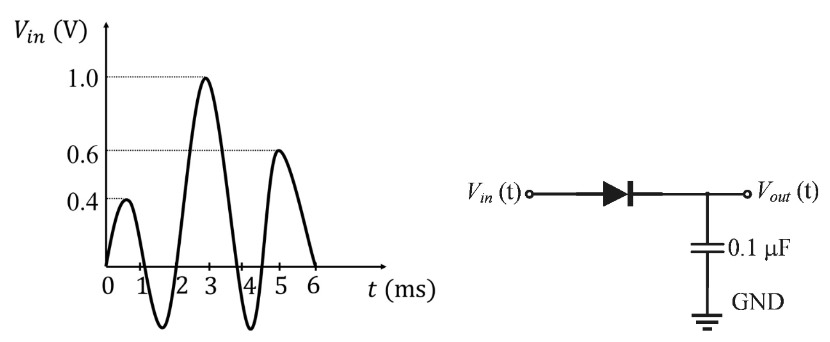
\includegraphics[width=1\linewidth]{2022/IN/36/figs/figuree.png} 
    \caption{ } 
\end{figure} 
\begin{enumerate} 
    \item 0.3V 
    \item0.6V 
    \item0.7V 
    \item1.0V 
\end{enumerate} 
\hfill(GATE 2022 IN 36)\\
\solution
\iffalse
\let\negmedspace\undefined
\let\negthickspace\undefined
\documentclass[journal,12pt,twocolumn]{IEEEtran}
\usepackage{cite}
\usepackage{amsmath,amssymb,amsfonts,amsthm}
\usepackage{algorithmic}
\usepackage{graphicx}
\usepackage{textcomp}
\usepackage{xcolor}
\usepackage{txfonts}
\usepackage{listings}
\usepackage{enumitem}
\usepackage{mathtools}
\usepackage{gensymb}
\usepackage{comment}
\usepackage[breaklinks=true]{hyperref}
\usepackage{tkz-euclide} 
\usepackage{listings}
\usepackage{gvv}                                        
\def\inputGnumericTable{}                                 
\usepackage[latin1]{inputenc}                                
\usepackage{color}                                            
\usepackage{array}                                            
\usepackage{longtable}                                       
\usepackage{calc}                                             
\usepackage{multirow}                                         
\usepackage{hhline}                                           
\usepackage{ifthen}                                           
\usepackage{lscape}
\usepackage{pgfplots}
\newtheorem{theorem}{Theorem}[section]
\newtheorem{problem}{Problem}
\newtheorem{proposition}{Proposition}[section]
\newtheorem{lemma}{Lemma}[section]
\newtheorem{corollary}[theorem]{Corollary}
\newtheorem{example}{Example}[section]
\newtheorem{definition}[problem]{Definition}
\newcommand{\BEQA}{\begin{eqnarray}}
\newcommand{\EEQA}{\end{eqnarray}}
\newcommand{\define}{\stackrel{\triangle}{=}}
\theoremstyle{remark}
\newtheorem{rem}{Remark}
\begin{document}

\bibliographystyle{IEEEtran}
\vspace{3cm}

\title{GATE 2022 IN 36}
\author{EE23BTECH11065 - prem sagar}
\maketitle
\newpage

\bigskip

\renewcommand{\thefigure}{\theenumi}
\renewcommand{\thetable}{\theenumi}
\textbf{Question}:
\\A signal $V_{in}\brak{t}$ shown is applied from t=0ms to t=6ms to the circuit shown Given the intial voltage across capacitor is 0.3V, and that the diode is ideal,the open circuit voltage $V_{out}\brak{t}$ at t=5ms is
\begin{figure}[h]
    \centering
    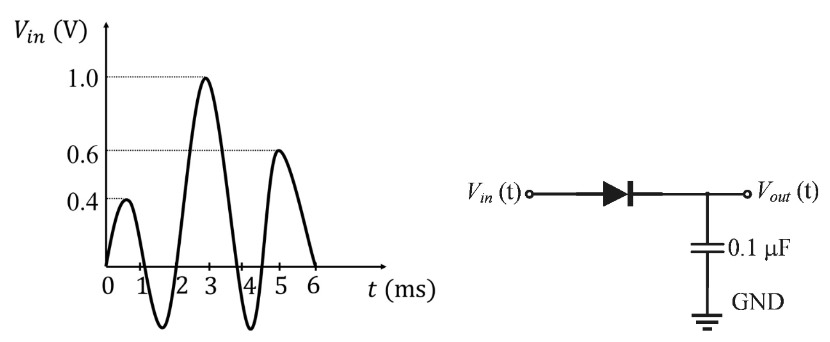
\includegraphics[width=1\linewidth]{2022/IN/36/figs/figuree.png}
    \caption{ }
\end{figure}
\begin{enumerate}
    \item 0.3V
    \item0.6V
    \item0.7V
    \item1.0V
\end{enumerate}
\hfill(GATE 2022 IN 36)
\\\textbf{Solution}:
\fi
\begin{table}[!ht]
\def\arraystretch{1.5}
   \centering
   \begin{tabular}{|c|c|c|}
    \hline
            \textbf{Symbol} & \textbf{Value} & \textbf{Description} \\
    \hline
          $V_{in}\brak{t}$ &  & input signal\\
    \hline
          $V_c\brak{t}$ &  & voltage across capacitor\\
    \hline 
          $V_c\brak{0}$ &$0.3$V &intial voltage across capacitor\\
    \hline
          $v_{out}\brak{t}$ & &open circuit voltage\\
    \hline  
    $V_D$    & &Voltage across diode\\
    \hline
    $I_D$& &Diode current \\
    \hline
    $I_S$& &Saturation current \\
    \hline
    $V_T$&$\frac{kt}{q}$ &Thermal voltage \\
    \hline
  \end{tabular}

    \caption{input parameters}
 \end{table}
\\ the circuit is a positive peak detector circuit  
\begin{align}
I_D&=I_S\brak{e^\frac{V_D}{V_T}-1}
\end{align}
At t=3ms; $V_D>0$
\\$\therefore$ diode is forward biased
\begin{align}
\\V_{out}\brak{t}&=V_c\brak{t}
\\&=1V
\end{align}
After $t>3$ms; $V_D<0$
\\$\therefore$ diode is reverse biased
\\the capacitor voltage remains at 1V  
\\$\therefore$ at t=5ms
\begin{align}
V_{out}\brak{t}&=1V
\end{align}
\\\begin{figure}[h]
\renewcommand\thefigure{1}
    \centering
    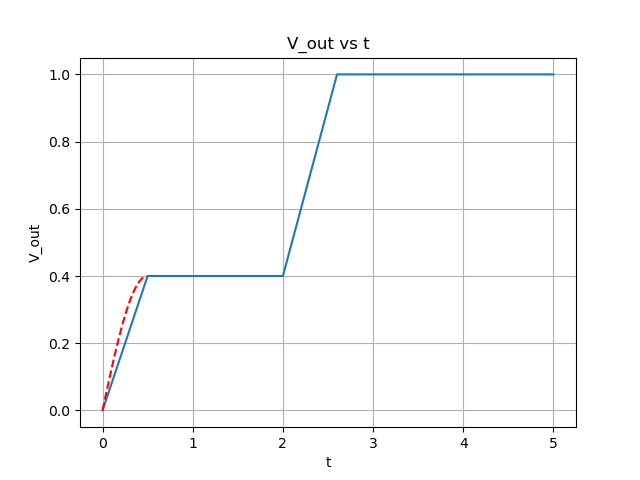
\includegraphics[width=1\linewidth]{2022/IN/36/figs/typo.png}
    \caption{ }
\end{figure}
%\end{document}

\pagebreak
\end{enumerate}
